\chapter[Pruebas y Resultados Experimentales]{Pruebas y Resultados Experimentales}

En este capitulo se presentan el funcionamiento del simulador para el estándar CAN J1939 y  las  pruebas de comunicación realizadas con dicho equipo para observar el funcionamiento del protocolo,  además, se presentan pruebas de comunicación realizadas con vehículos reales para el estándar OBD-II, logrando obtener datos de los sensores presentes, luego un análisis de las fallas presentadas durante las pruebas, y se concluye con el análisis financiero del desarrollo del producto.

\section{Simulador SAE J1939}

El simulador Au-SAE J1939 Versión 2.00A es un dispositivo capaz de proveer la mayoría de las señales de la norma SAE J1939. 
Una topología de red típica SAE J1939 se ilustra en la Figura~\ref{TPSAE} en dónde el simulador se conecta al bus mediante una resistencia interna de 120 ohmios, además trae consigo un conector RS-232 para utilizarlo con una Computadora en caso de ser necesario. 
Este simulador es proporcionado por la empresa Electrónica Au Grup para utilizarlo en las pruebas de sistemas SAE J1939, en la Figura~\ref{Sim} se observa su apariencia. 

\begin{figure}[H]
	\centering
		\includegraphics[width=0.8\textwidth]{./Cap6imagen/EjemploSimulador.pdf}
	\caption[Topología de Red SAE J1939.]{Topología de Red SAE J1939.\textbf{ Fuente:} \cite{UserM}.}
	\label{TPSAE} % Etiqueta para la referencia.
\end{figure}



\begin{figure}[H]
	\centering
		\includegraphics[width=0.8\textwidth]{./Cap6imagen/Simulador.png}
	\caption[Simulador BUS CAN SAE J1939.]{Simulador BUS CAN SAE J1939.\textbf{ Fuente:} \cite{UserM}.}
	\label{Sim} % Etiqueta para la referencia.
\end{figure}


\subsection {Principales Características del Simulador}
El simulador SAE J1939  está equipado con una resistencia de carga interna de 120 ohmios, Protección TVS(\textit{Transient Voltage Suppressor}, por sus siglas en inglés) para protección contra altos niveles de tensión, LED de encendidos, zumbador para indicar el funcionamiento y botones de configuración. 
El simulador tiene como entrada un conector DB9  para las conexiones CANH y CANL, además de la propia alimentación del dispositivo. 
Trabaja a 12V y puede consumir una corriente máxima de 250mA. 
Puede operar en dos modos llamados estáticos y dinámicos. 


\subsection{Modo de Funcionamiento}

Las simulaciones pueden ser operadas con sólo el control de los 3 botones presentes en el equipo. Con la configuración guiada por estos botones se genera una señal SAE J1939 para su uso en desarrollos de sistemas BUS CAN para camiones.

El equipo debe conectarse a una fuente externa entre 9-12 V. 
La alimentación se realiza con los pines 1 (Tierra) y 5 (Potencial positivo), la conexión del BUS CAN tanto CANH como CANL se realiza en los pines 6 y 7 como se muestra en la \textbf{Figura \ref{DB9}}.  
El indicador LED de encendido se ilumina y al estar listo el equipo emite un sonido a través del zumbador, entonces el simulador Au SAE J1939 empieza a funcionar en el modo (estático o dinámico) guardado en la última vez de su funcionamiento.

\begin{figure}[H]
	\centering
		\includegraphics[width=0.8\textwidth]{./Cap6imagen/SimDb9.pdf}
	\caption[Conector DB9 macho BUS CAN.]{Conector DB9 macho BUS CAN.\textbf{ Fuente:} \cite{UserM}.}
	\label{DB9} % Etiqueta para la referencia.
\end{figure}

El modo estático genera una señal SAE J1939 constante, los  dos pulsadores (Up y Down) se utiliza para cambiar las salidas de datos mediante la decisión del usuario. 
En el modo dinámico todos los datos SAE-J1939 cambian automáticamente sin que el rango de valores sea intervenido por el usuario del equipo. 
Para pasar de un modo de funcionamiento a otro se presiona los botones MENU y UP al mismo tiempo durante más de 1 segundo, es decir, para cambiar entre el modo dinámico y el modo estático. 
Una vez realizado, la confirmación del cambio se detecta con un zumbido del equipo.

En el modo estático el botón Down se utiliza para decrementar los valores de las señales SAE-J1939 presentes en las salidas del BUS CAN. 
Los LEDs muestran el descenso de las señales de manera porcentual, de la misma manera el botón Up se utiliza para aumentar los valores de las señales SAE-J1939 y los LEDs muestran el aumento de las señales de manera porcentual. 
la manera de cambiar entre estos dos modos se realiza presionando al mismo tiempo los botones MENÚ y UP por más de un segundo, de esta manera se intercala entre los modos de funcionamiento estático y dinámico. 
Un pitido largo será oído para reflejar la entrada de la tecla MENU y UP.

A modo de resumen se indica las funciones básicas de los botones:
\begin{itemize}
\item Botón DOWN: permite disminuir todos los datos simulados hasta que alcanza el valor más bajo.
 \item botón UP: permite aumentar todos los datos simulados hasta que alcanza el valor más alto.
\item MENÚ + UP: Cambia el funcionamiento del simulador entre el modo estático y dinámico.

\end{itemize}

\section{Pruebas Realizadas con el Simulador J1939}
Se realiza una prueba con el simulador y para ello conectamos un bus entre el hardware y el simulador J1939, alimentados ambos por una fuente de tensión de 12v. Como se observa en la Figura~\ref{simulador_ref_c6}

\begin{figure}[H]
	\centering
	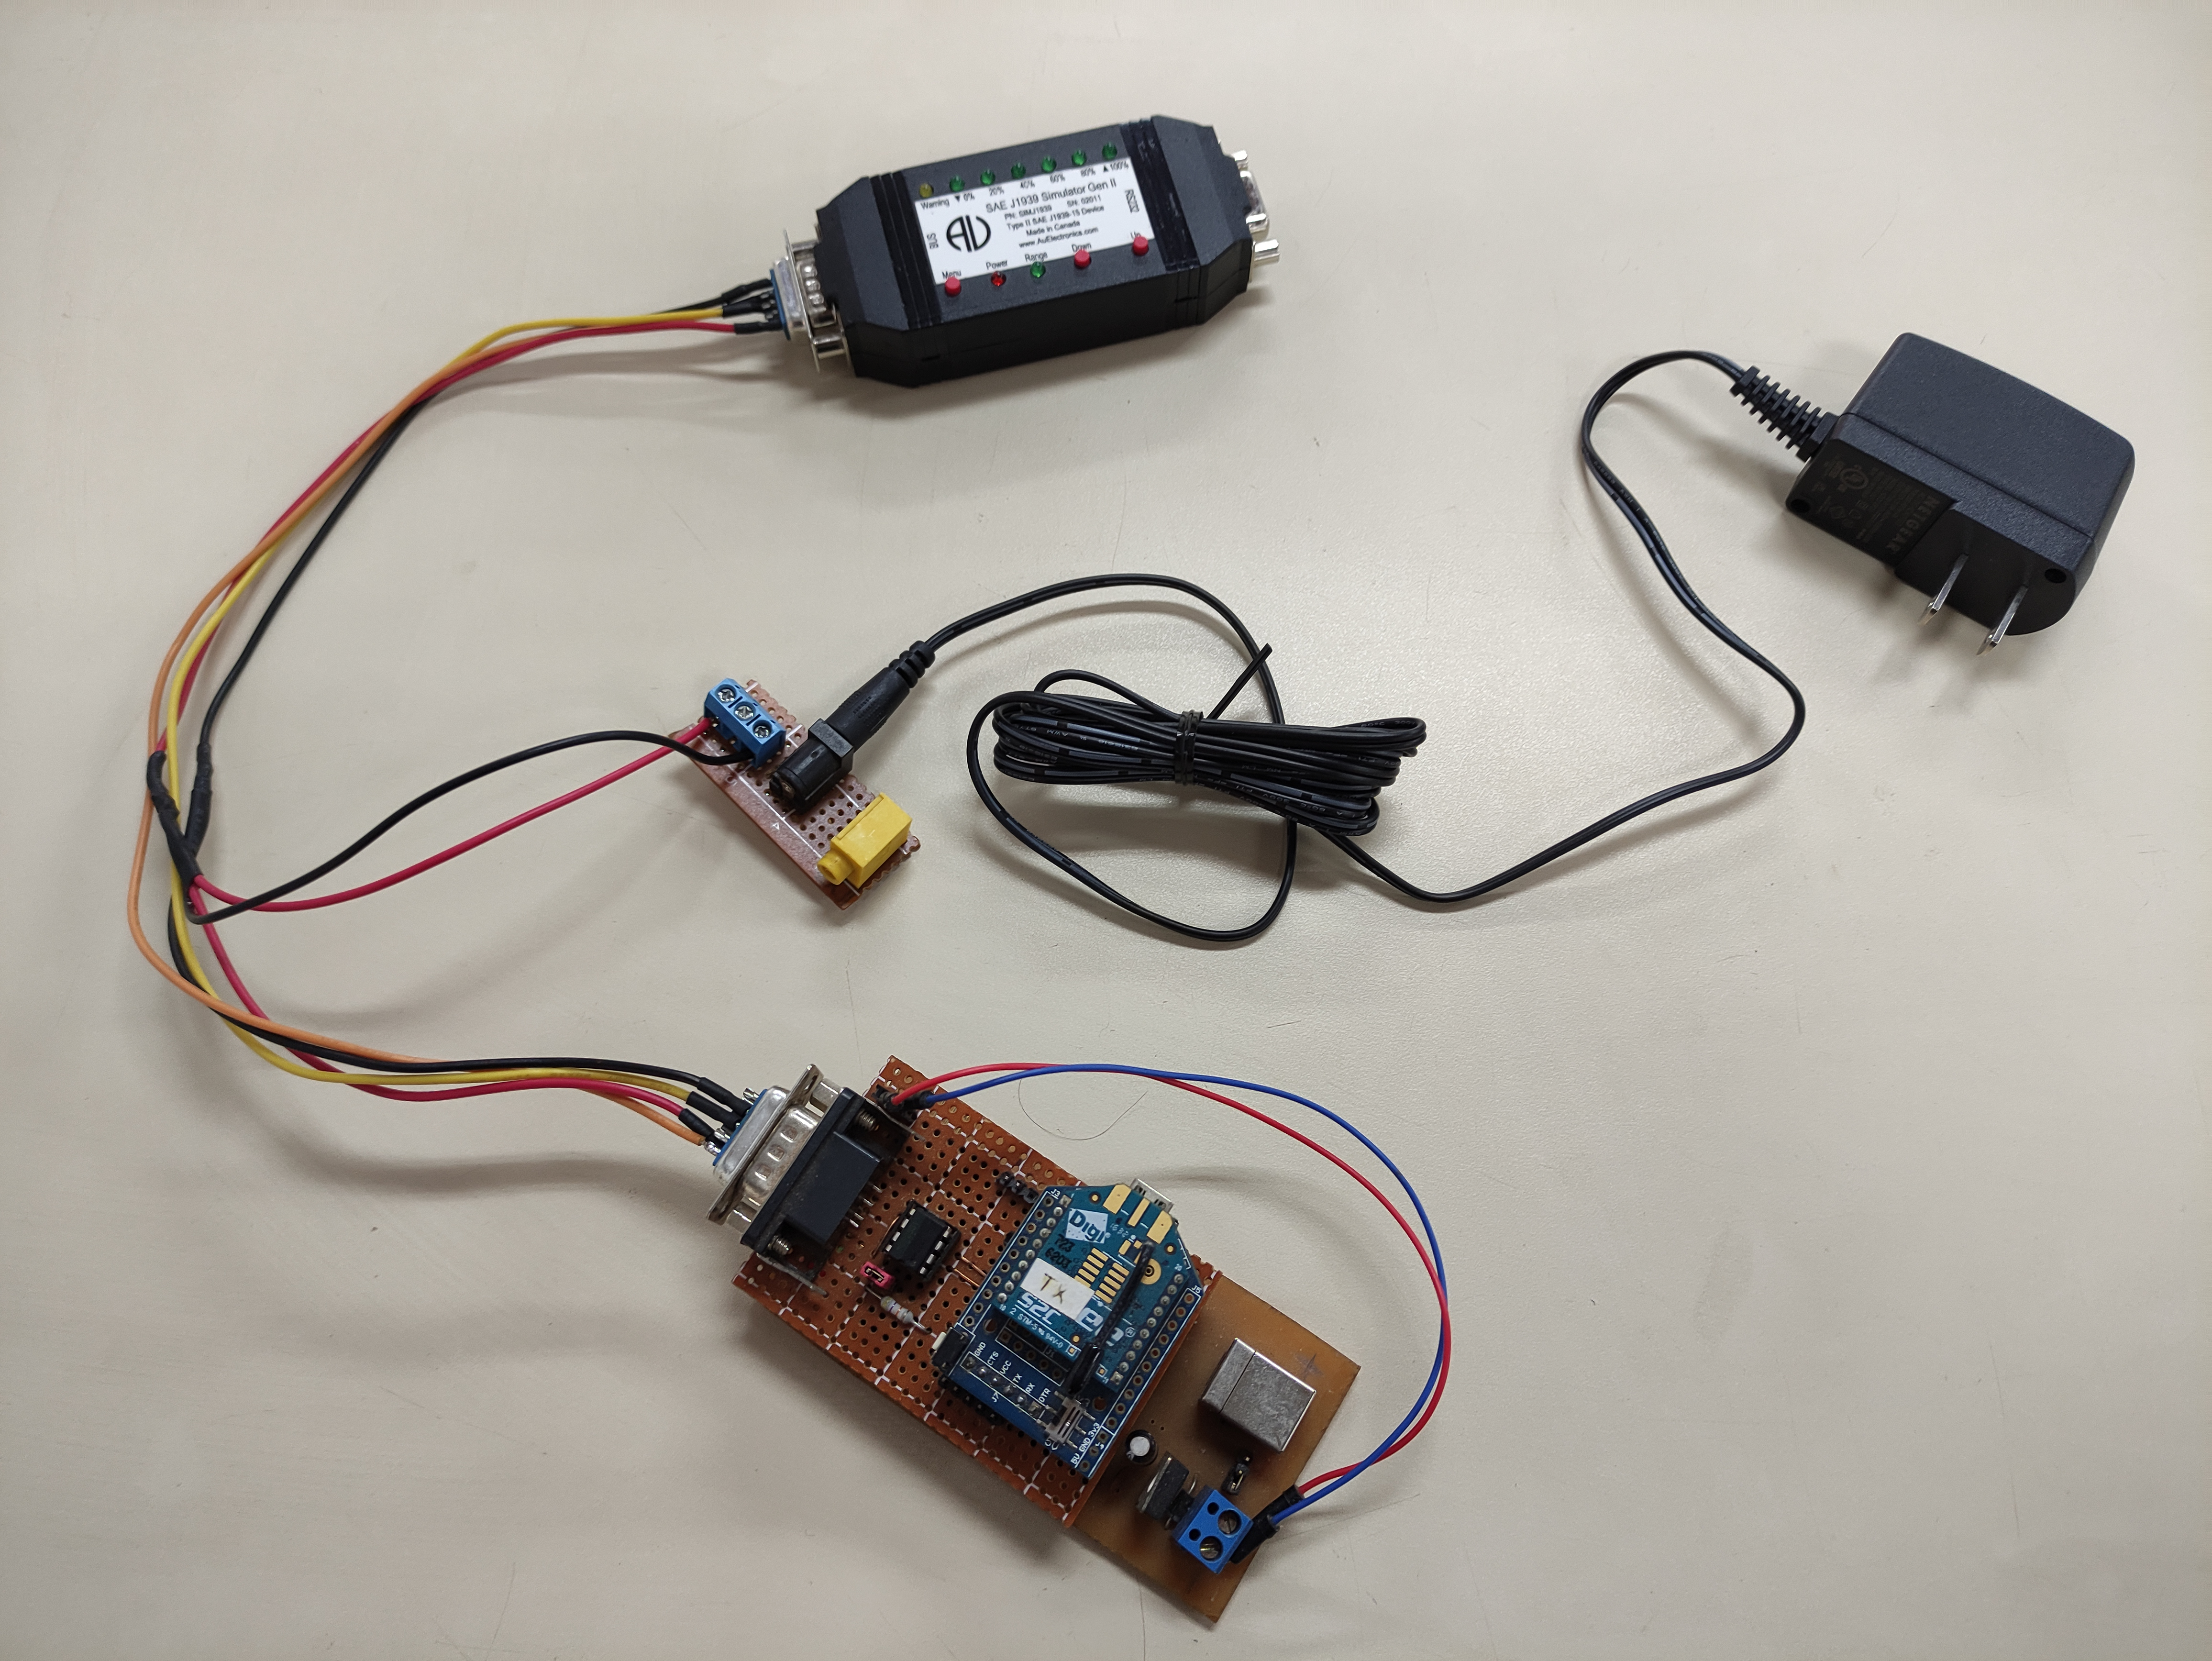
\includegraphics[width=0.5\textwidth]{./Cap6imagen/simulador_fig_c6.jpg}
	\caption [Conexión del Simulador J1939.]{Conexión del Simulador J1939 \textbf{ Fuente:} %\cite{cite_can_c3}.}
		Elaboración propia.}
	\label{simulador_ref_c6} % Etiqueta para la referencia.
\end{figure}

Se conecta el modulo Xbee receptor al puerto USB de la computadora y se inicia el software al acceder en la página web, Figura~\ref{receptor_ref_c6},  se selecciona el sistema J1939 y con el botón escucha se va recibiendo los datos enviados. 


\begin{figure}[H]
	\centering
	\includegraphics[width=0.5\textwidth]{./Cap6imagen/receptor_fig_c6.jpg}
	\caption [Receptor ubicado en el puerto USB.]{Receptor ubicado en el puerto USB \textbf{ Fuente:} %\cite{cite_can_c3}.}
		Elaboración propia.}
	\label{receptor_ref_c6} % Etiqueta para la referencia.
\end{figure}

Se selecciona la opción datos y observamos todas las tramas J1939 que está presente en el bus, aquí se puede observar la dirección de destino y origen de los dispositivos, los 8 bytes de datos en el cual los valores FF significa que dichos datos no están disponibles, pero los demás datos distintos a FF significan que son datos reales y disponibles, también podemos observar la prioridad de los mensajes que varía entre 3 y 6 según la Figura \ref{escucha_ref_c6}.

\begin{figure}[H]
	\centering
	\includegraphics[width=0.8\textwidth]{./Cap6imagen/escucha_fig_c6.png}
	\caption [Datos leídos del BUS CAN J1939.]{Datos leídos del BUS CAN J1939 \textbf{ Fuente:} %\cite{cite_can_c3}.}
		Elaboración propia.}
	\label{escucha_ref_c6} % Etiqueta para la referencia.
\end{figure}


También se puede observar la frecuencia de tipos de paquetes CAN presentes en el bus, en la Figura~\ref{paquetes_ref_c6}, los paquetes 0xF004 han sido recibidos 102 veces y los paquetes 0xFEF2 solamente 2 veces han sido captados. 
Hay varias tramas CAN que el simulador nos envía y mientras van apareciendo, el hardware los va captando y a su vez enviando al computador para su visualización. 
En el caso de la 


\begin{figure}[H]
	\centering
	\includegraphics[width=0.8\textwidth]{./Cap6imagen/paquetes_fig_c6.png}
	\caption [Tramas CAN J1939 presentes.]{Tramas CAN J1939 presentes \textbf{ Fuente:} %\cite{cite_can_c3}.}
		Elaboración propia.}
	\label{paquetes_ref_c6} % Etiqueta para la referencia.
\end{figure}


En la Figura~\ref{real_ref_c6} siguiente podemos observar la distribución de los datos aleatorios que van dejando el simulador en el bus, en este caso pertenece a la velocidad del vehículo. 
Se puede ver la forma en la cual el simulador distribuye los datos con el tiempo.  
Los datos van ingresando y el programa ajusta la gráfica para que quepan todos los datos y se pueda observar su comportamiento.  

\begin{figure}[H]
	\centering
	\includegraphics[width=0.8\textwidth]{./Cap6imagen/real_fig_c6.png}
	\caption [Datos de Velocidad del BUS CAN J1939.]{Datos de velocidad del BUS CAN J1939 \textbf{ Fuente:} %\cite{cite_can_c3}.}
		Elaboración propia.}
	\label{real_ref_c6} % Etiqueta para la referencia.
\end{figure}


En la Figura \ref{gauge_ref_c6} observamos una visualización en formato de tablero, para visualizar los datos manera familiar a la de un tablero de vehículo. 
Para obtenerlo, presionamos velocidad y luego activar, para poder filtrar de entre todas las tramas la trama que contiene los datos de la velocidad, se observa una captura de velocidad de 158 metros por segundo. 


\begin{figure}[H]
	\centering
	\includegraphics[width=0.8\textwidth]{./Cap6imagen/gauge_fig_c6.png}
	\caption [Tablero de Velocidad J1939.]{Tablero de velocidad J1939 \textbf{ Fuente:} %\cite{cite_can_c3}.}
		Elaboración propia.}
	\label{gauge_ref_c6} % Etiqueta para la referencia.
\end{figure}

\section{Pruebas realizadas en Vehículos con el sistema OBD II}

Para el sistema OBD II fue puesta a prueba el sistema en tres vehículos de las marcas Toyota 2019, Hyundai Creta 2021 y Hyundai Tucson 2011, en donde se realizó las medidas de distintos sensores para obtener datos de revoluciones por minuto del motor, voltaje de batería, velocidad y lectura de lista de sensores presentes en el vehículo,etc. 
Se puede ver en las Figuras \ref{auto_ref_c6}, \ref{creta_ref_c6} y \ref{tucson_ref_c6}  las imágenes de los tipos de vehículo automotor usados en las pruebas. 

\begin{figure}[H]
	\centering
	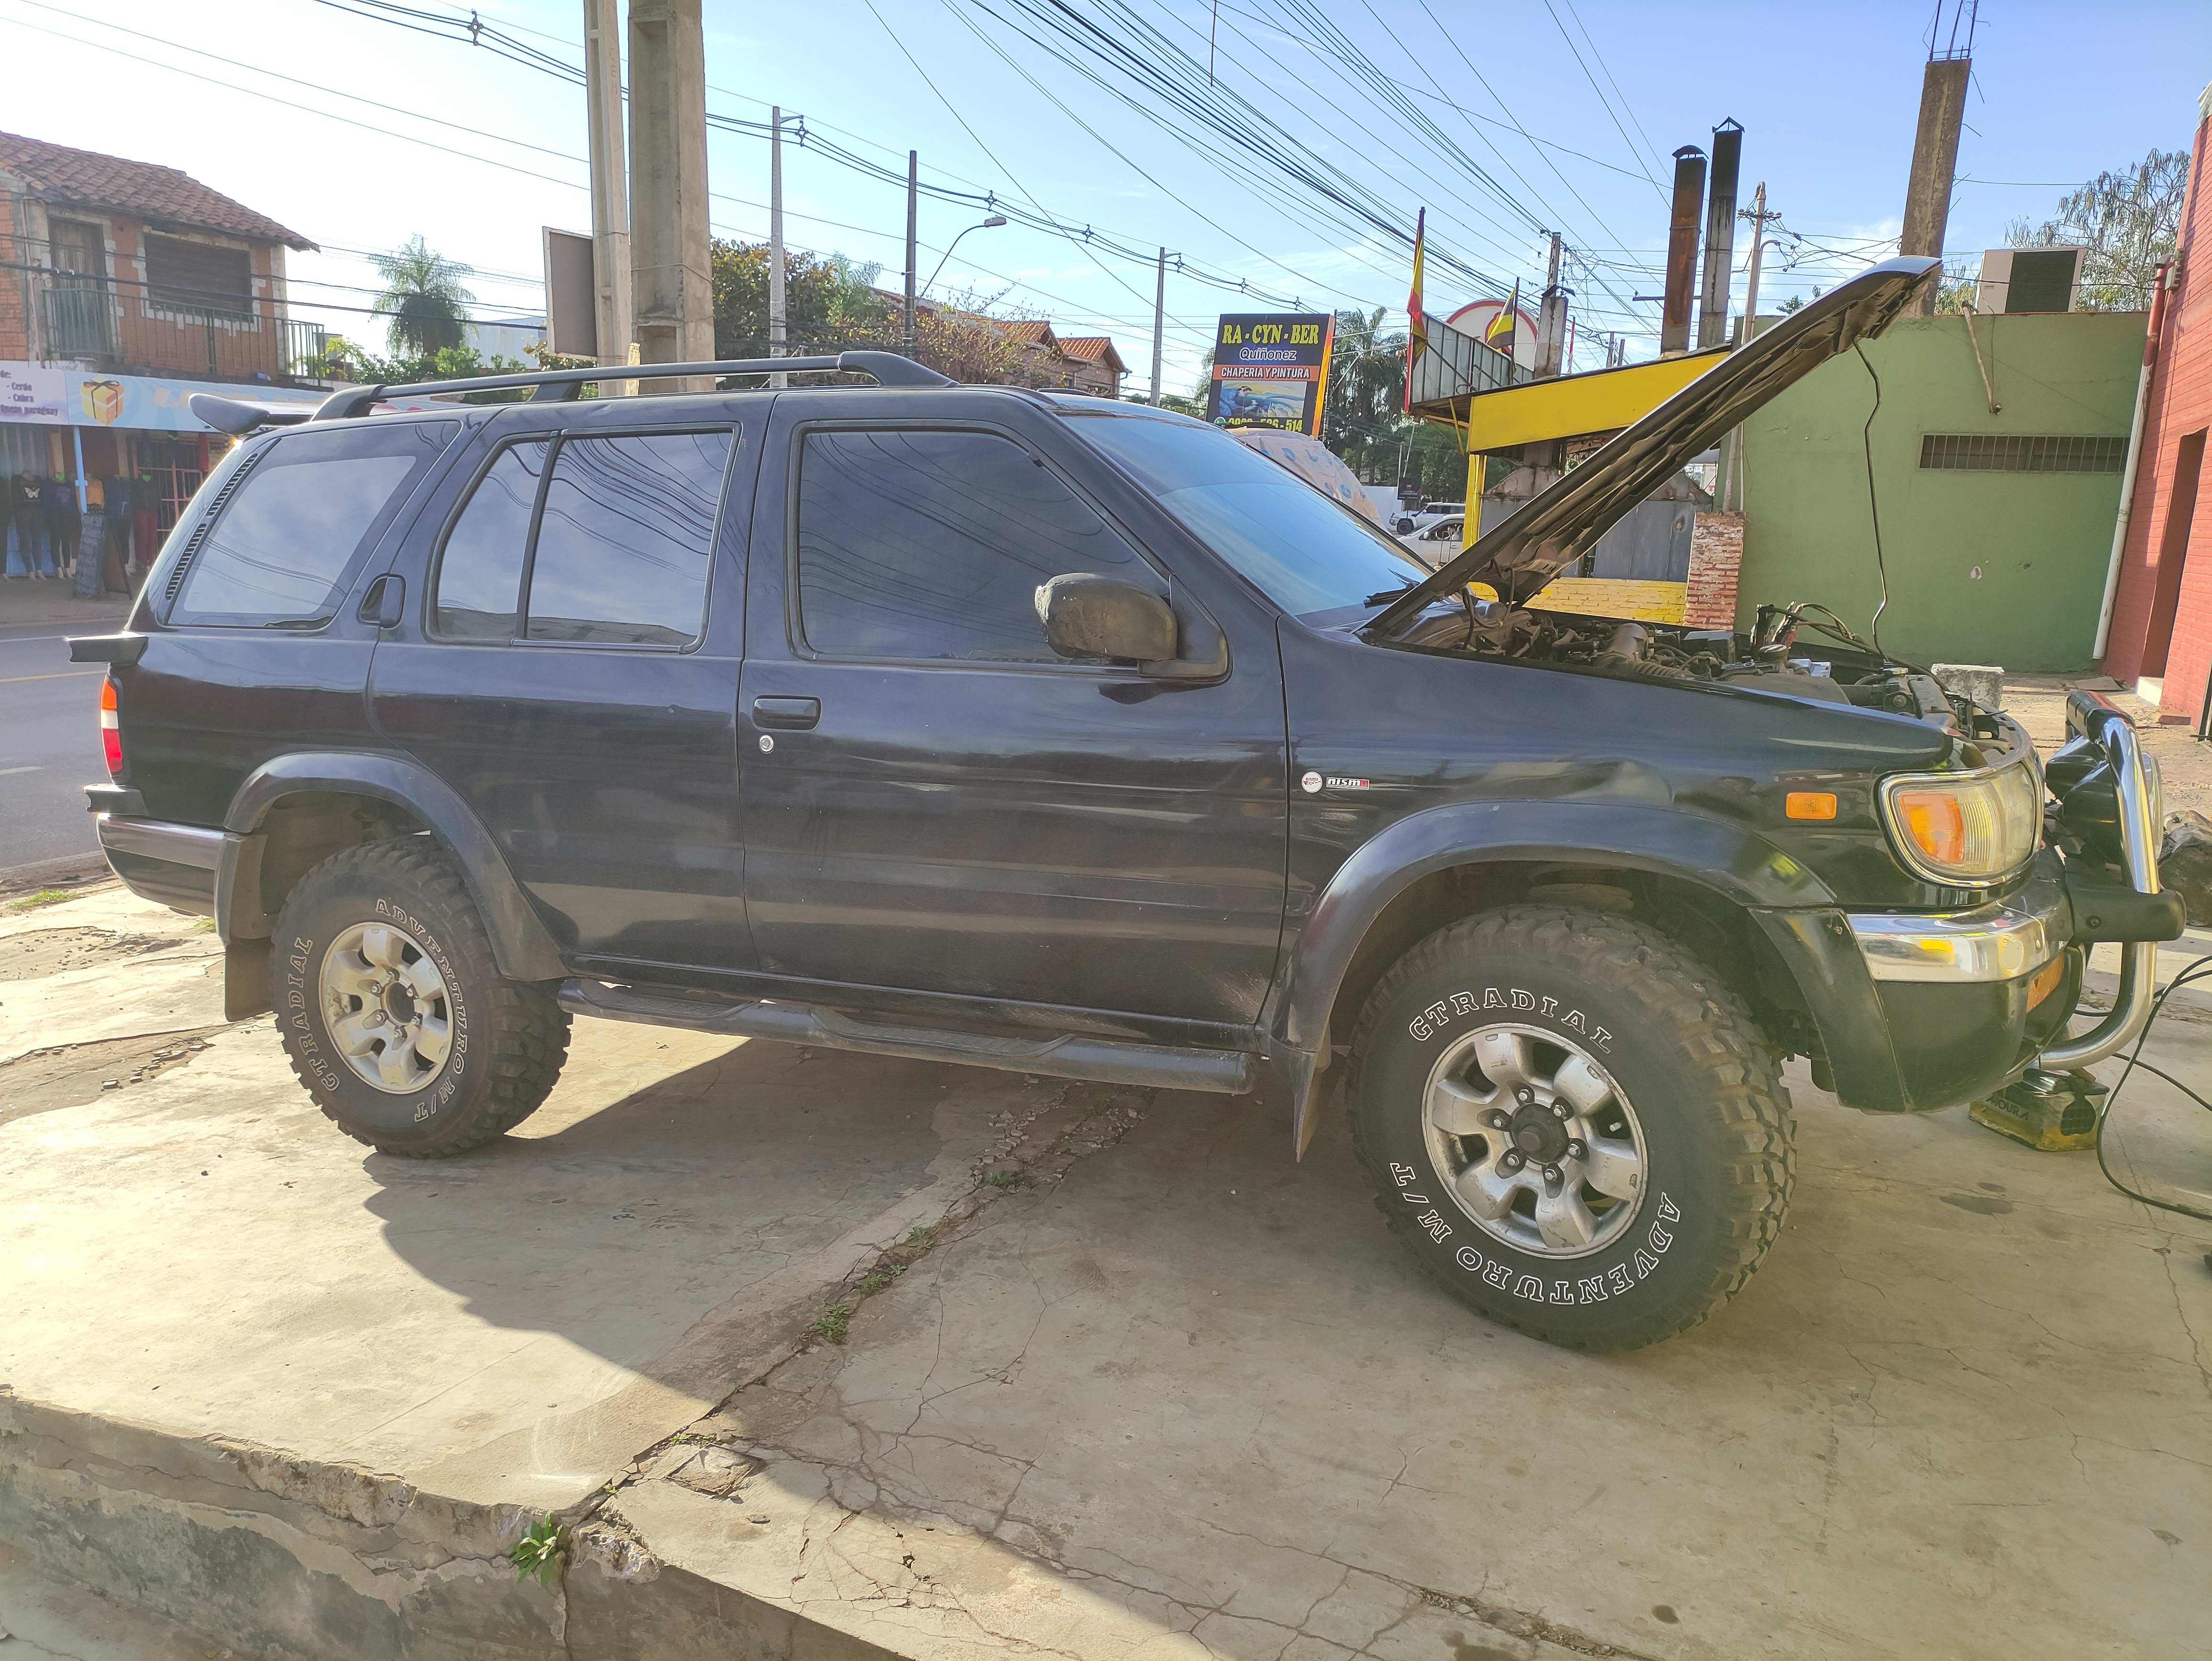
\includegraphics[width=0.8\textwidth]{./Cap6imagen/auto_fig_c6.jpg}
	\caption [Vehículo utilizado para la Prueba OBD II.]{Vehículo utilizado para la Prueba OBD II \textbf{ Fuente:} %\cite{cite_can_c3}.}
		Elaboración propia.}
	\label{auto_ref_c6} % Etiqueta para la referencia.
\end{figure}

\begin{figure}[H]
	\centering
	\includegraphics[width=0.8\textwidth]{./Cap6imagen/creta_fig_c6.jpg}
	\caption [Vehículo Creta 2021 utilizado para la Prueba OBD II.]{Vehículo Creta 2021 utilizado para la Prueba OBD II \textbf{ Fuente:} %\cite{cite_can_c3}.}
		Elaboración propia.}
	\label{creta_ref_c6} % Etiqueta para la referencia.
\end{figure}

\begin{figure}[H]
	\centering
	\includegraphics[width=0.8\textwidth]{./Cap6imagen/tucson_fig_c6.jpg}
	\caption [Vehículo Tucson 2011 utilizado para la Prueba OBD II.]{Vehículo Tucson 2011 utilizado para la Prueba OBD II \textbf{ Fuente:} %\cite{cite_can_c3}.}
		Elaboración propia.}
	\label{tucson_ref_c6} % Etiqueta para la referencia.
\end{figure}

En la Figura\ref{panel_ref_c6} observamos las consultas soportadas actualmente por el sistema, que son:
\begin{itemize}
    \item \textbf{Soportes PIDs}: presenta la lista de sensores del vehículo. 
    \item \textbf{Consulta PID}: sirve para consultar sensores que no soporta el sistema de visualización pero podemos leer la codificación. 
    \item \textbf{Revoluciones}: sirve para visualizar las revoluciones por minuto del motor vehicular.
    \item \textbf{Batería, Temperatura y velocidad} son otras visualizaciones soportadas.     
\end{itemize}



\begin{figure}[H]
	\centering
	\includegraphics[width=0.8\textwidth]{./Cap6imagen/soportes_fig_c6.png}
	\caption [Panel Principal OBD II.]{Panel Principal OBD II \textbf{ Fuente:} %\cite{cite_can_c3}.}
		Elaboración propia.}
	\label{panel_ref_c6} % Etiqueta para la referencia.
\end{figure}


En la Figura\ref{consola_ref_c6} se pueden ver en modo consola las lecturas de algunos sensores del vehículo Toyota como las revoluciones por minuto, velocidad, niveles de batería y otros. 
Para el momento de la captura de imagen el sistema indicaba mediciones de rpm (revoluciones por minuto) del motor. 

\begin{figure}[H]
	\centering
	\includegraphics[width=0.8\textwidth]{./Cap6imagen/consola_fig_c6.png}
	\caption [Datos recibidos del Vehículo.]{Datos recibidos del Vehículo \textbf{ Fuente:} %\cite{cite_can_c3}.}
		Elaboración propia.}
	\label{consola_ref_c6} % Etiqueta para la referencia.
\end{figure}


 Se realizó una lectura de medición de temperatura del aceite de motor en reposo, es decir, antes de arrancar el motor del vehículo, se observó la siguiente medición que se muestra en la Figura \ref{temp_ref_c6}. 
 La medida fue de 38 grados Celsius, la misma se presenta con un termómetro animado del lado izquierdo y el valor numérico del lado derecho.
 
 \begin{figure}[H]
	\centering
	\includegraphics[width=0.8\textwidth]{./Cap6imagen/temp_fig_c6.png}
	\caption [Visualización de la medida del sensor de temperatura de aceite del motor en reposo.]{Visualización de la medida del sensor de temperatura de aceite del motor en reposo \textbf{ Fuente:} %\cite{cite_can_c3}.}
		Elaboración propia.}
	\label{temp_ref_c6} % Etiqueta para la referencia.
\end{figure}

Otra medida de prueba fueron las revoluciones por minuto en estado de reposo, pero con el vehículo encendido, se observa en la Figura~\ref{rpm_ref_c6} la lectura obtenida de 872 rpm del motor del vehículo, nuevamente en dos formatos para una lectura familiarizada con el tablero analógico de un vehículo y otra digitalmente. 

\begin{figure}[H]
	\centering
	\includegraphics[width=0.8\textwidth]{./Cap6imagen/rpm_fig_c6.png}
	\caption [Visualización de la medida del sensor de revoluciones por minuto con el motor en reposo.]{Visualización de la medida del sensor de revoluciones por minuto con el motor en reposo.  \textbf{ Fuente:} %\cite{cite_can_c3}.}
		Elaboración propia.}
	\label{rpm_ref_c6} % Etiqueta para la referencia.
\end{figure}


Para el vehículo modelo \textbf{Tucson 2011} se realizaron las pruebas de: 


\begin{itemize}
    \item Lista de algunos sensores presentes en el vehículo
    \item Sensor de velocidad
    \item Voltaje de Batería en contacto marca una tensión de 12V y una vez encendido el motor marca una tensión de 14V, con lo cuál se puede concluir que son lecturas coherentes, pues el generador está activo y recargando la batería del vehículo. 
    \item Medida de revoluciones por minuto del motor en estado de reposo. 
    \item tiempo de encendido del motor
\end{itemize}

Algunas de estas  mediciones se muestran en la Figura \ref{dash_ref_c6}, además de una muestra por consola de los datos recibidos del hardware. 

\begin{figure}[H]
	\centering
	\includegraphics[width=0.8\textwidth]{./Cap6imagen/dash_fig_c6.jpg}
	\caption [Visualización de varias medidas de sensores.]{Visualización de varias medidas de sensores.  \textbf{ Fuente:} %\cite{cite_can_c3}.}
		Elaboración propia.}
	\label{dash_ref_c6} % Etiqueta para la referencia.
\end{figure}


El sistema provee una manera de leer los sensores que el hardware no tiene programado para hacerlo. 
Esto se realiza enviando el código PID deseado y  se traslada el calculo de la trama CAN al cliente. 
Para el ejemplo se realiza la lectura del temporizador del vehículo, el cual nos indica el tiempo que lleva encendido el automotor. 
Para ello se consulta el documento SAE J1979, se observa el código PID y la formula requerida de lectura del temporizador. 
Estos datos se introducen en el sistema mediante la interfaz gráfica, Figura~\ref{consulta_ref_c6}, una vez presionado el botón \"activar\", el software dibuja  una gráfica en el tiempo de los valores de la consulta. 
En la Figura~\ref{grafica_ref_c6} se observa la lectura del temporizador en el tiempo indicando que el automóvil lleva encendido 650 segundos. 

\begin{figure}[H]
	\centering
	\includegraphics[width=0.8\textwidth]{./Cap6imagen/consulta_fig_c6.png}
	\caption [Visualización de varias medidas de sensores.]{Visualización de varias medidas de sensores.  \textbf{ Fuente:} %\cite{cite_can_c3}.}
		Elaboración propia.}
	\label{consulta_ref_c6} % Etiqueta para la referencia.
\end{figure}

\begin{figure}[H]
	\centering
	\includegraphics[width=0.8\textwidth]{./Cap6imagen/grafica_fig_c6.jpg}
	\caption [Visualización de varias medidas de sensores.]{Visualización de varias medidas de sensores.  \textbf{ Fuente:} %\cite{cite_can_c3}.}
		Elaboración propia.}
	\label{grafica_ref_c6} % Etiqueta para la referencia.
\end{figure}

Para el automotor modelo Creta 2021 además de leer los mismos datos anteriores, se realizó una prueba en movimiento para medir los datos de los sensores de velocidad. 
La lectura se visualiza en la Figura \ref{vel_ref_c6} en dónde se compara con el tablero del vehículo.

\begin{figure}[H]
	\centering
	\includegraphics[width=0.9\textwidth]{./Cap6imagen/vel_fig_c6.png}
	\caption [Comparación de la medida de Velocidad en un vehículo Creta 2021.]{Comparación de la medida de Velocidad en un vehículo Creta 2021.  \textbf{ Fuente:} %\cite{cite_can_c3}.}
		Elaboración propia.}
	\label{vel_ref_c6} % Etiqueta para la referencia.
\end{figure}

Con estas pruebas se lograron la lectura de los sensores básicos presentes en los vehículos. 

\section{Inconvenientes encontrados en las Pruebas}

Durante las pruebas han sido necesario ajustar algunos parámetros y se ha encontrado otras dificultades enunciadas a continuación: 
\begin{itemize}
    \item Ha sido necesario ajustar el bit denominado RTR en el módulo del protocolo CAN, cuyo valor estándar es 1 (uno) y tuvo que ser cambiado a 0 (cero) para la comunicación. El bit RTR es el encargado de solicitar una trama CAN a los dispositivos en la red, se observó que los estándares J1939 y OBD-II no implementan el bit RTR, por lo que se ajustó su valor a cero. 
    
    \item La mayoría de los autos presentaban fallas de comunicación por avería del conector OBD-II o el propio sistema. Esto se comprobó con un escáner vehicular comercial. 
    
    \item Algunos automóviles  no contaban con el protocolo CAN, sino con otros tipos de protocolos, como la ISO 14230-4 KWP. No todos los vehículos  implementan el protocolo CAN actualmente. 
    
\end{itemize}


El escáner vehicular utilizado para la comprobación  y comparación del funcionamiento del sistema CAN desarrollado se muestra en la Figura~\ref{scaner_fig_c6}: 

\begin{figure}[H]
	\centering
	\includegraphics[width=0.6\textwidth]{./Cap6imagen/scaner_fig_c6.png}
	\caption [Escáner de la Marca Launch CRP123.]{Escáner de la Marca Launch CRP123.  \textbf{ Fuente:} %\cite{cite_can_c3}.}
		Elaboración propia.}
	\label{scaner_fig_c6} % Etiqueta para la referencia.
\end{figure}

\section[Análisis Financiero]{Análisis Financiero}

\subsection{Costos del Hardware y Software desarrollados}
En el proyecto se analizaron los gastos teniendo en cuenta  recursos materiales y humanos utilizados. 
Para el calcular el proceso de esfuerzo humano se realizó un promedio del salario en base a un desarrollador de software en Paraguay. 
Como el proyecto está hecho con lenguajes de programación web para el software y lenguaje C para el hardware se vio que los Desarrolladores web y multimedia ganan normalmente un salario neto mensual aproximado de entre Gs. 3.000.000 y Gs. 6.000.000 al empezar en el puesto de trabajo, esto según las referencias obtenidas de la página tusalario.org,~\cite{tusalario}, así haciendo un promedio y suponiendo 20 días de trabajo al mes con 8 horas diarias, el costo por horas de trabajo es de 30 000Gs por hora aproximadamente. 
Se aborda este salario para el trabajo en \textit{backend}, \textit{frontend}, desarrollo de hardware y su programación. 
Como no se trabaja las 8 horas diarias por el desarrollo del sistema, empleamos 4 horas diarias para el desarrollo y las restantes 4 horas para otras gestiones e investigaciones que no carga con las horas del diseño en sí. 

En la Tabla~\ref{tabla:hw} se observa el costo de los componentes utilizados para el hardware, además de las herramientas utilizadas para su elaboración. 


%%%%%%%%%%%%%%%%%%%%% tabla %%%%%%%%%%%%%%%%%%%%%%%%%%%%%%%%
\begin{table}[H]
\begin{center}
\begin{tabular}{c l l r r }
\toprule
\textbf{Cant} & \textbf{Componente} & \textbf{Descripción} &\textbf{Unidad Gs.}&\textbf{Importe Gs.}  \\ 
\midrule
2    & Capacitores      & 10uF        & 250            & 500   \\ 
%\hline
2    & Capacitores      & 0,1uF       & 250            & 500   \\ 
%\hline
2    & Capacitores      & 15pf        & 1.000           & 2.000  \\ 
%\hline
1    & Resistor         & 330 ohm     & 250            & 250   \\ 
%\hline
1    & Resistor         & 100k        & 250            & 250   \\ 
%\hline
1    & Microcontrolador &PIC18F4580   & 85.000          & 85.000 \\ 
%\hline
1    & Regulador        & 7805        & 15.000          & 15.000 \\ 
%\hline
2    & Diodo            & 1N4148      & 1.000           & 2.000  \\ 
%\hline
1    & Diodo Led        & Rojo        & 1.000           & 1.000  \\ 
%\hline
1    & Botón            & 4 pines    & 3.500           & 3.500  \\ 
%\hline
1    & Conector        & DB9    & 5.000           & 5.000  \\ 
%\hline
1    & Espadines       & 5 pines   & 3.500           & 3500  \\ 
%\hline
2    & Módulo          & SHIELD & 55.000          & 110.000 \\ 
%\hline
2    & Módulo          & XBEE        & 250.000         & 500.000 \\ 
%\hline
2    & Espadines       & 20 pines  & 3.500           & 7.000    \\ 
%\hline
1    & Módulo          & MCP2551     & 30.000          & 30.000  \\ 
%\hline
1    & Cristal         & 16Mhz     & 5.000           & 5.000   \\ 
%\hline
1    & Placa de Cobre  & 1 Capa      & 13.000          & 13.000   \\ 
%\hline
1    & Conector OBD II  & OBD II     & 50.000          & 50.000   \\ 
%\hline
1    & Impresora 3D         & Caja 3D       & 100.000         & 100.000 \\ 
%\hline
1    & Fresadora CNC    & CNC        & 100.000         & 100.000 \\ 
%\hline
      &                  &            & \textbf{Total} & \textbf{1.033.500}  \\ 
      \bottomrule
\end{tabular}
\caption{Costo de los componentes y herramientas usadas en el hardware.}
\label{tabla:hw}
\end{center}
\end{table}

Para el desarrollo del proyecto se organizó el trabajo en 4 partes:  diseño del hardware, programación del hardware, Programación del Software \textit{frontend} (Diseño de Usuario) y Programación del software \textit{backend} (Programación del servidor), cada uno con un costo de 30.000 Gs/hora-hombre y un tiempo total de 1120hs. repartidas en las distintas etapas del desarrollo, como se aprecia en la Tabla~\ref{tabla:software} con sus costos correspondientes. 

%%%%%%%%%%%%%%%%%%%%% tabla %%%%%%%%%%%%%%%%%%%%%%%%%%%%%%%%
\begin{table}[H]
\begin{center}
\begin{tabular}{l r r r}
\toprule
\textbf{Trabajo Realizado} & \textbf{Horas}&\textbf{Salario por hora Gs.} & \textbf{Importe Gs.} \\ \hline

 Placa Electrónica & 160 & 30.000  & 4.800.000     \\ 
 %\hline
 Software CAN      & 320 & 30.000  & 9.600.000     \\ 
 %\hline
 Diseño de Usuario & 320 & 30.000  & 9.600,000     \\ 
 %\hline
 Programación del Servidor & 320 & 30.000 & 9.600.000 \\ 
 %\hline 
 \textbf{ Total } & \textbf{1120} & & \textbf{33.600.000} \\ %\hline 
\bottomrule
\end{tabular}
\caption{Tabla Costos de mano de obra.}
\label{tabla:software}
\end{center}
\end{table}
%%%%%%%%%%%%%%%%%%%%%%%%%%%%%%%%%%%%%%%%%%%%%%%%%%%%%%%%%%%%%%%%%%%%



En la Tabla \ref{tabla:licencias} observamos el costo de las licencias de Proteus~\cite{licenp}, y el compilador PIC CCS~\cite{pic_ccs}.
%%%%%%%%%%%%%%%%%%%%% tabla %%%%%%%%%%%%%%%%%%%%%%%%%%%%%%%%
%%%% \textbf{tabla \ref{tabla:hw}} 
\begin{table}[H]
\begin{center}
\begin{tabular}{l l r }
\toprule
\textbf{Herramienta} & \textbf{Licencia} & \textbf{Costo}  \\ 
\midrule
Proteus Starter Kit  & Básica & 1.600.000  \\ 
Compilador PIC CCS   & PIC18  & 1.400.000  \\ 
\textbf{Total Costos} &  &   3.000.000     \\ \bottomrule
\end{tabular}
\caption{Tabla Costos de Licencias.}
\label{tabla:licencias}
\end{center}
\end{table}
%%%%%%%%%%%%%%%%%%%%%%%%%%%%%%%%%%%%%%%%%%%%%%%%%%%%%%%%%%%%%%%%


En la Tabla \ref{tabla:total} presentamos el costo total del proyecto teniendo en cuenta los resultados de las tablas anteriores: 

%%%%%%%%%%%%%%%%%%%%% tabla %%%%%%%%%%%%%%%%%%%%%%%%%%%%%%%%
%%%% \textbf{tabla \ref{tabla:hw}} 
\begin{table}[H]
\begin{center}
\begin{tabular}{l r}
\toprule
\textbf{Referencia} & \textbf{Costos}  \\ 
\midrule
Costos Hardware  & 1.033.500\\ 
%\hline
Costos Mano de Obra  & 33.600.000     \\ 
%\hline
Costos Licencias & 3.000.000\\ 
%\hline
\textbf{Total Costos} & 37.633.500    \\ 
%\hline
\bottomrule
\end{tabular}
\caption{Tabla costos totales.}
\label{tabla:total}
\end{center}
\end{table}
%%%%%%%%%%%%%%%%%%%%%%%%%%%%%%%%%%%%%%%%%%%%%%%%%%%%%%%%%%%%%%%%

Así el costo mínimo del proyecto sería de 37.633.500 Gs. cayendo la mayor parte del costo en la mano de obra humana para la elaboración del sistema, es decir, el 89\% del costo recae en el capital humano y solo el 11\% recae en los costos materiales y licencias. 

\subsection{Mejoras Futuras del Hardware y del Sistema}

Con más tiempo de desarrollo y con un presupuesto mas alto se podría diseñar mejoras al prototipo del sistema al complementarlo con una computadora Raspberry Pi con la posibilidad de convertirse en un servidor de datos para otros puntos de acceso.
Por ejemplo: que una vez conectado el módulo CAN al vehículo, otros dispositivos como computadoras y celulares puedan acceder a los datos leídos mediante una red o por sistemas como wifi o bluetooth, al mismo tiempo que el propio dispositivo despliega los datos en una propia pantalla, de esta manera se tendría versatilidad en su uso.

Para las herramientas de software se podría optar por usar software \textit{open source} para el diseño del hardware como Kicad~\cite{kitcad} y para el compilador utilizar el ''Standard-Eval Version" de Microchip~\cite{compmicro}, cuya única limitación sería que la optimización del compilador es de pago, pero si el proyecto utiliza poca memoria no sería obstáculo usarlo en la versión libre, ya que no tenemos tiempo crítico. 

En la Fig~\ref{fig_raspberri_c4} se observa la propuesta con tres bloques de funcionamiento. 
En el \textbf{bloque 1} el hardware CAN se conectaría al vehículo y se encargaría de las lecturas del sistema, así mediante bluetooth se conectaría al \textbf{bloque 2} con la Raspberry Pi, el cual sería responsable de la visualización de los datos. 
Hasta aquí se tendría un sistema CAN OBD II completo, pero adicionalmente en el \textbf{bloque 3} se muestra como el software del proyecto está preparado para conectarse a una red de internet para que otros dispositivos tengan acceso a los datos del vehículo, el módulo Wifi o el puerto Ethernet ya está incorporado en la Raspberry Pi para esta funcionalidad. 

%%%%%%%%%%%%%%%%%%%%%%%%%%%%%%%%%%%%%%%%%%%%%%%%%%%%%%%%%%
\begin{figure}[H]
	\centering
		\includegraphics[width=0.9\textwidth]{./Cap00imagen/fig_raspberri_f.png}
	\caption[Sistema CAN con raspberry Pi.]{Sistema CAN con raspberry Pi.\textbf{ Fuente:}  Elaboración Propia.}
	\label{fig_raspberri_c4} % Etiqueta para la referencia.
\end{figure}

% CITAR IMAGEN
%%%%%%%%%%%%%%%%%%%%%%%%%%%%%%%%%%%%%%%%%%%%%%%%%%%%%%%%%%

Para reducir el tamaño físico de hardware CAN se presupuesta usar componentes electrónicos de montajes superficiales y agregar un módulo bluetooth para la conexión con la computadora Raspberry Pi, el presupuesto aproximado de la fabricación completa se logró obtener con la ayuda de la empresa PCBway~\cite{pcbway}, ya que posee unos pasos a seguir para el cálculo de presupuesto para la fabricación completa de un circuito PCB con los componentes incluidos. 
En la Tabla~\ref{tabla:raspberri} se muestran el presupuesto del hardware para este nuevo sistema.
%%%%%%%%%%%%%%%%%%%%% tabla %%%%%%%%%%%%%%%%%%%%%%%%%%%%%%%%
\begin{table}[H]
\begin{center}
\begin{tabular}{ l l r}
\toprule
\textbf{Elementos} & \textbf{Comentario} & \textbf{Costo}  \\ 
\midrule
Hardware CAN    & PCB Fabricado    & 918.000 \\ %\hline
Conector        & OBD II - J1939     & 50.000 \\ %\hline
Módulo          & Bluetooth          & 60.000 \\ %\hline
Computadora     & Raspberry PI 4    & 600.000 \\ %\hline
Pantalla TFT    & 4 pulgadas         & 300.000 \\ %\hline
Protector       & Caja 3D            & 150.000\\ %\hline
\textbf{Total Costos}&  &2 078 000 \\ 
%\hline
\bottomrule


\end{tabular}
\caption{Costo de los elementos para una propuesta mejorada del sistema CAN.}
\label{tabla:raspberri}
\end{center}
\end{table}


Podemos recurrir al software del anterior proyecto y realizar una adaptación del mismo a la Raspberry Pi y modificar el código del microcontrolador para trabajar con el módulo bluetooth, esto agregaría horas de trabajo pero ya no serían tantas si se aprovecha el proyecto original, así en la Tabla~\ref{tabla:extra} se observa los costos de adaptación siguiendo los mismos precios de 30.000 Gs/hora-hombre para el trabajo y una cantidad de 240 horas de trabajo distribuida en las distintas partes del proyecto.  

%%%%%%%%%%%%%%%%%%%%% tabla %%%%%%%%%%%%%%%%%%%%%%%%%%%%%%%%
\begin{table}[H]
\begin{center}
\begin{tabular}{l r r r}
\toprule
\textbf{Trabajo Realizado} & \textbf{Horas}&\textbf{Salario por hora Gs.} & \textbf{Importe Gs.} \\ 
\midrule
 Placa Electrónica & 80 & 30 000  & 2.400.000     \\ 
 Software CAN      & 160  & 30.000  & 4.800.000     \\ 
 Diseño de Usuario & 80  & 30.000  & 2.400.000     \\ 
 Programación del Servidor & 80 & 30.000 & 2.400.000 \\ 
  \textbf{Total } & \textbf{240}  &  & \textbf{12.000.000} \\ \bottomrule
\end{tabular}
\caption{Tabla Costos de mano de obra.}
\label{tabla:extra}
\end{center}
\end{table}
%%%%%%%%%%%%%%%%%%%%%%%%%%%%%%%%%%%%%%%%%%%%%%%%%%%%%%%%%%%%%%%%%%%%



En la \textbf{tabla \ref{tabla:nuevototal}} presentamos el costo total del proyecto teniendo en cuenta los resultados de las tablas anteriores: 

%%%%%%%%%%%%%%%%%%%%% tabla %%%%%%%%%%%%%%%%%%%%%%%%%%%%%%%%
%%%% \textbf{tabla \ref{tabla:hw}} 
\begin{table}[H]
\begin{center}
\begin{tabular}{l r}
\toprule
\textbf{Referencia} & \textbf{Costos}  \\ 
\midrule
Costos Hardware  & 2.078.000     \\ 
Costos Mano de Obra  & 12.000.000     \\ 
Costos Licencias &         0     \\ 
\textbf{Total Costos} & 14.078.000    \\ 
\bottomrule
\end{tabular}
\caption{Tabla costos totales para el nuevo sistema CAN.}
\label{tabla:nuevototal}
\end{center}
\end{table}
%%%%%%%%%%%%%%%%%%%%%%%%%%%%%%%%%%%%%%%%%%%%%%%%%%%%%%%%%%%%%%%%

Rediseñar el sistema aprovechando la primera versión costaría un agregado de 14 078 000 Gs. que es un \textbf{37\%} del costo total del proyecto original. 